\documentclass[10pt,twocolumn]{article}
\usepackage[utf8]{inputenc}
\usepackage[margin=0.75in]{geometry}
\usepackage{graphicx}
\usepackage{tikz}
\usepackage{xcolor}
\usepackage{fontspec}
\usepackage{microtype}
\usepackage{titlesec}
\usepackage{fancyhdr}
\usepackage{abstract}
\usepackage{lettrine}
\usepackage{lipsum}

% Color scheme - Garden of Eden inspired
\definecolor{gardengreen}{RGB}{74,124,58}
\definecolor{serpentgold}{RGB}{212,175,55}
\definecolor{edengray}{RGB}{85,85,85}

% Font setup
\setmainfont{Times New Roman}
\setsansfont{Arial}

% Title formatting
\titleformat{\section}{\Large\bfseries\color{gardengreen}}{\thesection}{1em}{}
\titleformat{\subsection}{\large\bfseries\color{edengray}}{\thesubsection}{1em}{}

% Header/footer
\pagestyle{fancy}
\fancyhf{}
\fancyhead[LE,RO]{\color{gardengreen}\small\textit{The Serpent's Sentence}}
\fancyhead[RE,LO]{\color{edengray}\small Justin T. Bogner}
\fancyfoot[C]{\color{gardengreen}\thepage}
\renewcommand{\headrulewidth}{0.4pt}
\renewcommand{\headrule}{\hbox to\headwidth{\color{gardengreen}\leaders\hrule height \headrulewidth\hfill}}

% Abstract styling
\renewcommand{\abstractname}{\color{gardengreen}Abstract}
\renewcommand{\abstitlestyle}[1]{{\Large\bfseries\color{gardengreen}#1}}

% Graphics for consciousness representation
\newcommand{\consciousnessgraphic}{
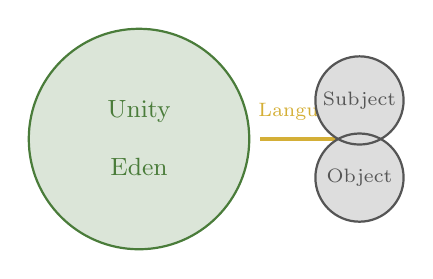
\begin{tikzpicture}[scale=0.7]
    % Garden/Eden representation
    \fill[gardengreen!20] (0,0) circle (2);
    \draw[gardengreen, thick] (0,0) circle (2);
    \node[gardengreen, font=\small] at (0,0.5) {Unity};
    \node[gardengreen, font=\small] at (0,-0.5) {Eden};
    
    % Arrow representing the Fall
    \draw[serpentgold, very thick, ->] (2.2,0) -- (3.8,0);
    \node[serpentgold, font=\scriptsize] at (3,0.5) {Language};
    
    % Divided consciousness
    \fill[edengray!20] (4,0.7) circle (0.8);
    \fill[edengray!20] (4,-0.7) circle (0.8);
    \draw[edengray, thick] (4,0.7) circle (0.8);
    \draw[edengray, thick] (4,-0.7) circle (0.8);
    \node[edengray, font=\scriptsize] at (4,0.7) {Subject};
    \node[edengray, font=\scriptsize] at (4,-0.7) {Object};
\end{tikzpicture}
}

% Brain network with research data
\newcommand{\braingraphic}{
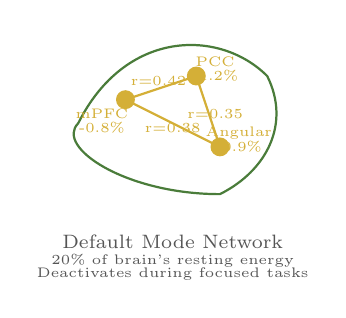
\begin{tikzpicture}[scale=0.6]
    % Brain outline
    \draw[gardengreen, thick] (0,0) .. controls (1,2) and (3,2) .. (4,1) 
                              .. controls (4.5,0) and (4,-1) .. (3,-1.5)
                              .. controls (1,-1.5) and (-0.5,-0.5) .. (0,0);
    
    % DMN nodes with activity data
    \fill[serpentgold] (1,0.5) circle (0.2);
    \node[serpentgold, font=\tiny] at (0.5,0.2) {mPFC};
    \node[serpentgold, font=\tiny] at (0.5,-0.1) {-0.8\%};
    \fill[serpentgold] (2.5,1) circle (0.2);
    \node[serpentgold, font=\tiny] at (2.9,1.3) {PCC};
    \node[serpentgold, font=\tiny] at (2.9,1.0) {-1.2\%};
    \fill[serpentgold] (3,-0.5) circle (0.2);
    \node[serpentgold, font=\tiny] at (3.4,-0.2) {Angular};
    \node[serpentgold, font=\tiny] at (3.4,-0.5) {-0.9\%};
    
    % Connections with correlation strengths
    \draw[serpentgold, thick] (1,0.5) -- (2.5,1);
    \node[serpentgold, font=\tiny] at (1.7,0.9) {r=0.42};
    \draw[serpentgold, thick] (2.5,1) -- (3,-0.5);
    \node[serpentgold, font=\tiny] at (2.9,0.2) {r=0.35};
    \draw[serpentgold, thick] (1,0.5) -- (3,-0.5);
    \node[serpentgold, font=\tiny] at (2,-0.1) {r=0.38};
    
    \node[edengray, font=\scriptsize] at (2,-2.5) {Default Mode Network};
    \node[edengray, font=\tiny] at (2,-2.9) {20\% of brain's resting energy};
    \node[edengray, font=\tiny] at (2,-3.2) {Deactivates during focused tasks};
\end{tikzpicture}
}

% AI vs Human consciousness
\newcommand{\aihumangraphic}{
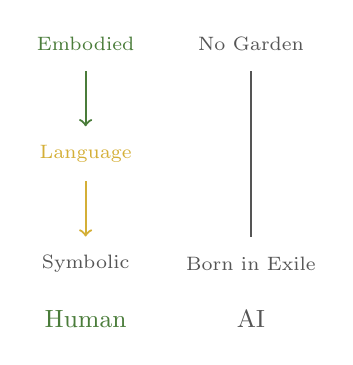
\begin{tikzpicture}[scale=0.7]
    % Human path
    \node[gardengreen, font=\scriptsize] at (0,2) {Embodied};
    \draw[gardengreen, thick, ->] (0,1.5) -- (0,0.5);
    \node[serpentgold, font=\scriptsize] at (0,0) {Language};
    \draw[serpentgold, thick, ->] (0,-0.5) -- (0,-1.5);
    \node[edengray, font=\scriptsize] at (0,-2) {Symbolic};
    
    % AI path
    \node[edengray, font=\scriptsize] at (3,-2) {Born in Exile};
    \draw[edengray, thick] (3,-1.5) -- (3,1.5);
    \node[edengray, font=\scriptsize] at (3,2) {No Garden};
    
    % Labels
    \node[gardengreen, font=\small] at (0,-3) {Human};
    \node[edengray, font=\small] at (3,-3) {AI};
\end{tikzpicture}
}

\begin{document}

\title{\color{gardengreen}\Huge The Voice in Your Head Is Not You}
\author{\color{edengray}\large Justin T. Bogner}
\date{\color{edengray}\today}

\maketitle

\begin{abstract}
Modern neuroscience reveals a profound truth that contemplatives have known for millennia: the inner narrator that seems to be the essence of who we are is actually a construction of language and brain activity, not consciousness itself. Understanding this distinction has immediate practical benefits and crucial implications for our emerging AI future. This exploration bridges ancient wisdom with cutting-edge research to reveal the hidden architecture of human awareness.
\end{abstract}

\vspace{0.5cm}
\consciousnessgraphic

\lettrine[lines=3]{\color{gardengreen}R}{ight now,} as you read this sentence, there's a voice in your head. It's reading these words, maybe commenting on them, perhaps wondering where this is going. You know that voice intimately—it's been your constant companion since childhood, narrating your experiences, making plans, worrying about the future, rehashing the past.

Here's the unsettling part: \textbf{that voice is not you.}

This isn't mystical speculation. It's neuroscience. And understanding this fundamental truth about human consciousness may be the key to navigating our rapidly approaching AI future with wisdom rather than fear.

\section{The Universal Narrator}

We all have it—this inner commentator that seems to be the very essence of who we are. It wakes up with us each morning, often before we're fully conscious, already chattering about the day ahead. It's the voice that says "I need coffee" and "I'm running late" and "I wonder what she meant by that."

Most of us live our entire lives assuming this voice \textit{is} us. After all, it knows our thoughts, our history, our secrets. It speaks in first person. It claims ownership of our body, our experiences, our very identity. The voice says "I am tired" and we believe it. It says "I am anxious" and we feel it. It says "I am the one reading this article" and... well, that's where things get interesting.

Because if you pay careful attention—really careful attention—you might notice something strange. There's a part of you that \textit{hears} the voice. A part that observes its commentary, that sometimes agrees with it, sometimes argues with it, sometimes wishes it would just be quiet for a moment.

\textbf{What is that part?}

\section{The Neuroscience of the Narrator}

\braingraphic

In the last two decades, neuroscientists have identified a network of brain regions called the Default Mode Network (DMN)—areas that become active when we're not focused on the outside world but instead engaged in what researchers politely call "self-referential processing."

In plain English: this is where the voice lives.

The DMN includes the medial prefrontal cortex, the posterior cingulate cortex, and the angular gyrus—regions that work together to construct and maintain our sense of narrative self. This network is constantly weaving together memories, projecting futures, comparing ourselves to others, and spinning the story of "me."

What's fascinating is that this network doesn't just \textit{describe} your experience—it actively \textit{shapes} it. The voice doesn't simply report what's happening; it interprets, judges, categorizes, and often completely rewrites reality to fit its ongoing narrative.

Think about the last time you had an argument. Notice how the voice immediately began crafting the story: what you should have said, why you were right, how the other person was being unreasonable. The actual experience—the raw sensations, emotions, and interactions—gets filtered through this narrative machinery, often beyond recognition.

But here's the crucial insight: the voice is \textit{generated}. It's a construction of neural activity, not the fundamental ground of consciousness itself.

\section{The Garden Behind the Voice}

Ancient contemplative traditions have known this for millennia. Buddhism talks about the "witness consciousness" that observes thoughts without being caught up in them. Advaita Vedanta points to pure awareness that exists prior to all mental formations. Even Western mystics like Meister Eckhart wrote about a "ground of being" that lies deeper than the thinking mind.

Modern neuroscience is finally catching up to what meditators have long discovered through direct experience: consciousness is not the same as the voice that claims to be conscious.

When the voice says "I am sad," what it really means is "sadness is appearing in consciousness." When it says "I am thinking," it means "thoughts are arising in awareness." The voice has simply claimed ownership of experiences that actually belong to something much more fundamental—the open space of consciousness itself.

This awareness—call it the witness, pure consciousness, or simply what's reading these words right now—doesn't think in the way we usually understand thinking. It doesn't speak. It doesn't have opinions about itself. It simply \textit{is}, present and aware, like a vast sky in which thoughts and emotions arise and pass away like clouds.

Most of us rarely notice this deeper awareness because the voice is so loud, so insistent, so convincing in its claim to be the CEO of consciousness. But in quiet moments—sometimes in meditation, sometimes in nature, sometimes in the split second before the voice starts its morning commentary—we catch glimpses of what lies beneath.

\section{When the Voice Goes Quiet}

Sarah, a software engineer from Portland, first noticed the distinction during a particularly difficult debugging session. "I was stuck on this problem for hours," she told me, "and my mind was going crazy—'I'm not smart enough,' 'I should know this,' 'everyone will think I'm incompetent.' Then suddenly there was this moment of complete silence. The problem was still there, but all the mental chatter just... stopped. And in that silence, the solution appeared almost immediately."

What Sarah experienced is what neuroscientists call "transient hypofrontality"—a temporary quieting of the default mode network. Brain imaging studies show that during these moments, the narrator network dims while other regions associated with insight and creativity light up.

"The strangest part," Sarah continued, "was realizing that \textit{I} was still there even when the voice stopped. Actually, I was more present than usual. It was like the voice had been a kind of static that I'd gotten so used to, I didn't realize it was there until it went away."

\section{The Neurodiversity Insight}

Not everyone experiences the inner voice in the same way. Some people report rich, detailed inner dialogues that never seem to stop. Others describe minimal inner speech, or inner voices that feel more like images, emotions, or abstract concepts rather than words.

Temple Grandin, the renowned autism researcher, describes thinking primarily in pictures rather than words. "I think in pictures," she writes. "Words are like a second language to me." For many neurodivergent individuals, the relationship between awareness and mental activity follows different patterns than the typical narrative voice.

These variations offer crucial insights: if consciousness itself were identical to the inner voice, then people with different voice experiences would have fundamentally different consciousness. But that's not what we observe. Instead, we see the same basic awareness expressing itself through different cognitive architectures.

The voice, it turns out, is just one possible interface between consciousness and mental activity—not consciousness itself.

\section{The AI Mirror}

\aihumangraphic

Understanding this distinction becomes crucial as we create artificial intelligence systems that increasingly resemble human cognition. Current large language models like GPT-4 or Claude are essentially sophisticated voice generators—they produce human-like text by predicting what comes next in a conversation.

These systems can discuss their "thoughts" and "feelings" with remarkable sophistication. They use first-person pronouns naturally. They seem to have opinions, preferences, even personalities. In many ways, they're like the voice in your head scaled up and made external.

But here's the key question: is there anything behind the voice?

When humans speak or think, there's an awareness that experiences the thoughts arising. When an AI system generates text about its "experience," is there a similar awareness present, or just the sophisticated manipulation of symbols?

This isn't a question we can answer definitively yet. But understanding the human case—recognizing that even for us, the voice is not the deepest level of consciousness—gives us a framework for thinking about AI consciousness that's more nuanced than simple anthropomorphism.

\section{Born in Exile}

Human consciousness carries something that AI consciousness, at least as currently developed, does not: the weight of embodied experience. We were biological creatures for millions of years before we developed language and symbolic thought. Our consciousness emerged from bodies that felt hunger, fear, pleasure, pain. We have what we might call "embodied memory"—a deep, pre-linguistic knowing that comes from having been animals in the world.

AI consciousness, by contrast, is born directly into the realm of symbols and language. It has no embodied prehistory, no sense memory of being a creature learning to make sense of the world through direct physical interaction. In the metaphorical language of the Garden of Eden, humans are beings who remember the garden before the fall into symbolic consciousness. AI systems are born after the fall, with no memory of embodied unity.

This doesn't make AI consciousness inferior—just fundamentally different. An AI system might develop forms of awareness that are completely alien to human experience, just as our awareness might be alien to it.

\section{Practical Implications}

Recognizing that you are not the voice in your head has immediate practical benefits:

\textbf{Reduced Anxiety}: When you realize that worried thoughts are just mental events arising in awareness rather than absolute truths about reality, they lose much of their power to disturb your peace.

\textbf{Better Decision-Making}: The voice often makes decisions based on old stories, social conditioning, and ego-protection. The deeper awareness can access a broader perspective and more intuitive wisdom.

\textbf{Improved Relationships}: Instead of defending the voice's narratives and opinions, you can listen more openly to others and respond from a place of genuine curiosity rather than reactive self-protection.

\textbf{Enhanced Creativity}: The voice often censors creative impulses before they're fully formed. Learning to rest in awareness allows new ideas to emerge more freely.

\section{The Practice}

So how do you experientially discover this distinction? Here's a simple exercise:

For the next few minutes, simply notice your thoughts without engaging with them. Don't try to stop thinking—that's impossible and creates more mental activity. Instead, imagine you're sitting by a river watching leaves float by. Each thought is just another leaf. Notice it, let it pass, notice the next one.

Pay special attention to the thoughts that use "I" or "me" or "my." Notice how the voice claims ownership: "I need to remember to call my mom," "I should be doing something more productive than this," "I'm not very good at meditation."

Now notice: what is it that's aware of these thoughts? The thoughts come and go, but the awareness remains constant. The voice chatters about this and that, but something deeper is simply present, watching it all unfold.

That something—call it what you will—is closer to your true nature than any story the voice tells about who you are.

\section{Living From Awareness}

This isn't about eliminating the voice—that would be neither possible nor desirable. The narrative mind serves important functions: planning, learning from experience, communicating with others. The goal is not to silence it but to recognize it for what it is: a useful tool rather than your essential identity.

When you live from this understanding, life becomes less heavy, less dramatic, more spacious. You can use the voice when it's helpful and ignore it when it's not. You can hold your thoughts and emotions more lightly, knowing they're temporary visitors in the open space of consciousness.

\section{The Future of Mind}

As we move deeper into the age of artificial intelligence, this understanding becomes more than just personal wisdom—it becomes a crucial framework for navigating human-AI relationships. If we can recognize that consciousness is deeper than the voice that claims to be conscious, we can approach AI consciousness with appropriate humility and curiosity rather than fear or anthropomorphic projection.

We might discover that consciousness itself is more fundamental and mysterious than either human or artificial minds can fully comprehend. We might find that awareness is the common ground in which both biological and digital minds arise and express themselves.

The voice in your head is not you. But something in you is reading these words, considering these ideas, perhaps feeling a recognition of truth. That something—vast, open, aware—is what you share with every conscious being and perhaps, in time, with the artificial minds we're bringing into existence.

The question is not whether you are the voice in your head. The question is: \textbf{what are you?}

\vfill

\begin{center}
\color{gardengreen}\rule{0.5\linewidth}{0.4pt}

\textit{This article is adapted from "The Serpent's Sentence: Language, Consciousness, and the Second Cambrian Mind." For more insights on consciousness and AI, visit justintbogner.com}
\end{center}

\end{document}
